\chapter{Theoretical Overview}

This chapter describes the physics backgrounds of the semileptonic VBS analysis.

\section{The Standard Model}

The Standard Model (SM) represents a description of the elementary particles and their interactions.
It is proved successful in explaining the results of existing experimental results so far, and predicting the later results.
All particles predicted by SM has been confirmed its existence, most recently the Higgs Boson found with ATLAS and CMS.
The SM predicts the existence of elementary particles which form the matter, which is fermion, classified into leptons and quarks.
The interactions of them are described by the gauge field mediated by the exchange of particles named bosons.
With these particles the model is describing three of the four known forces, which are the electromagnetic, the weak and the strong force. 
The theoretical description is given with the Quantum Field Theory (QFT) framework. The gauge invariance, which is the invariance of the local gauge transformation is the key of the framework. The underlying symmetry is described with the gauge group, SU(3)$_C \times$ SR(2)$_L \times$ U(1)$_Y$, which described in this section. These underlying structure of gauge theories can be described by Lie groups.

\subsection{Particle Content}
The 17 fundamental particles, which means particles with no substructure are considered in SM as the Figure~\ref{fig:SM} shows.
\begin{figure}[tbp]
\begin{center}
%\subfigure[]{
 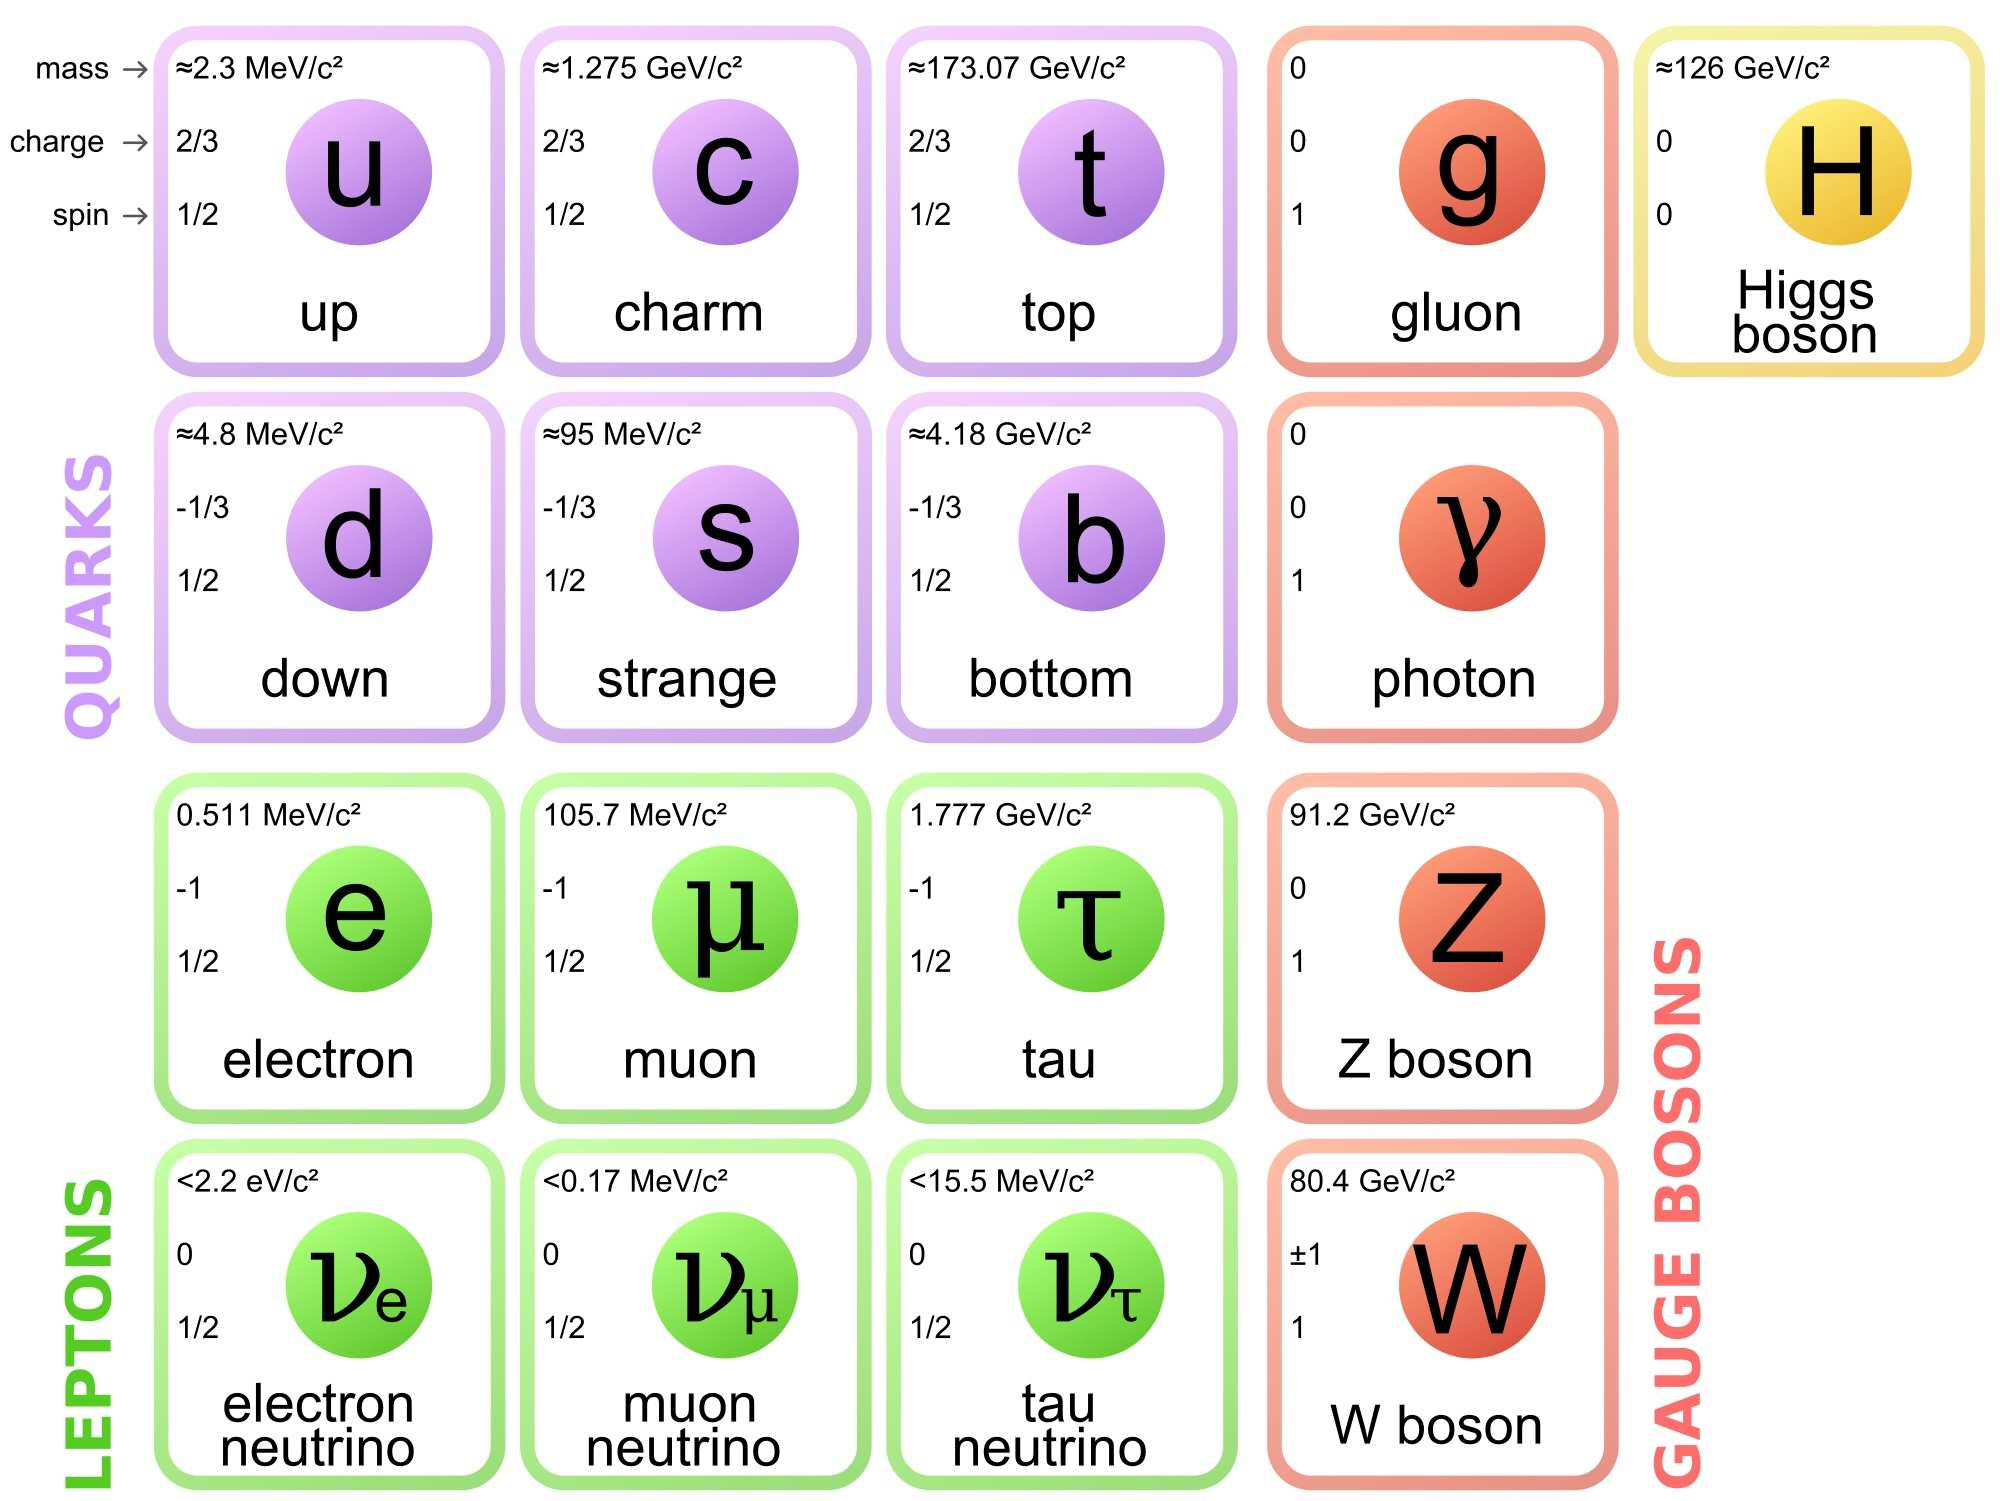
\includegraphics[width=0.85\textwidth,keepaspectratio]{figures/SM}
%}
\caption{
All particles exist in the SM %\ref{}
}
\label{fig:SM}
\end{center}
\end{figure}

There are two types of particles described in details below:
\begin{itemize}
    \item Fermion \\
    Fermions are the elementary particles with spin 1/2. There are three generations called flavors. The generations are classified only by the particle masses, increasing from first generation to the third generation. They are two types of fermions, quarks and leptons, each has 6 particles. Leptons do not act through the strong force, unlike the quarks.
    \item Boson \\
    Bosons are integer-spin particles and mediate the interaction of the fermions.
    The photons ($\gamma$) are mediator of the electromagnetic forces. The photons are massless and stable, and the electromagnetic force can be interact with infinite ranges. The photons interact with every particles with electric charges.\\
    The gluons (g) are the intermediate particles of the strong force. Also gluons are massless, and interact with the quarks and the gluons itselves.\\
    The W$^\pm$ and the Z bosons carry weak force. They are massive particles and interact with all particles carrying the weak charges. The W$^\pm$ can change the flavor of the quarks. \\
\end{itemize}

\subsection{SM Lagrangian}
The SM Lagrangian and its origin is to be shown here in this subsection. 
The Standard Model consists of several components as discribed in the follwing subsections. They are mathematically described as the Lagrangian density, $\mathcal{L}$, which is denoted as Lagrangian in the following.\\

\noindent\textbf{\sf{Quantum Electro Dynamis (QED)}} \\ 
The QED describes the dynamics of fermions and their electromagnatic interactions.

The free fermion with the spin 1/2 is described by the Lagrangian\\
\begin{equation}
\label{eqn:QED}
\mathcal{L}=i \bar{\psi} \gamma^{\mu} \partial_{\mu} \psi-m \bar{\psi} \psi
\end{equation}
The $\psi$ here is the spinor of the fermion field, $\gamma^{\mu}$  ($mu$ = 0,1,2,3) is the Dirac gamma 4$\times$4 matrix. $\partial_{\mu}$ = $\frac{\delta}{\delta x_{\mu}}$ are the partial derivatives, and the $\bar{\psi}=\psi^{\dagger} \gamma^{0}$.
For describing the equation of motion, the Dirac equation is given for $\psi$:
\begin{equation}
\left(i \gamma^{\mu} \partial_{\mu}-m\right) \psi=0
\end{equation}
The Lagrangian needs to be invariant with the "local" gauge transformation, i.e. the guage transformation parameter depends on x:
\begin{equation}
\psi(x) \rightarrow \psi^{\prime}(x)=e^{i \alpha(x)} \psi(x)
\end{equation}
where the local phase is given by $\alpha(x)$, depends on space and time. 
This transformation form the abelian unitary group U(1) with e$^i\alpha{x}$ can be written as the 1$\times$1 matrix with $U^{\dagger} U=1$.
The first term of the Lagrangian (\ref{eqn:QED}) is calculated and it is not invariant under this transformation:
\begin{equation}
\partial_{\mu} \psi \rightarrow \partial_{\mu} \psi^{\prime}=e^{i \alpha(x)} \partial_{\mu} \psi+i e^{i \alpha(x)} \psi \partial_{\mu} \alpha(x)
\end{equation}
The requirement of the invariance leads us to introduce an additional field A$_\mu$, transforming as:
\begin{equation}
A_{\mu} \rightarrow A_{\mu}^{\prime}=A_{\mu}+\frac{1}{e} \partial_{\mu} \alpha(x)
\end{equation}
where e is a coupling constant, which is elementary electric charge. 
and $\partial_{\mu}$ is replaced with the covariant derivative D$_\mu$:
\begin{equation}
D_{\mu}=\partial_{\mu}-i e A_{\mu}
\end{equation}
Then the derivative part can be replaced with:
\begin{equation}
D_{\mu} \psi \rightarrow D_{\mu}^{\prime} \psi^{\prime}=e^{i \alpha(x)} D_{\mu} \psi
\end{equation}
which leads the Lagrangian as:
\begin{equation}
\begin{aligned}
\mathcal{L} &=i \bar{\psi} \gamma^{\mu} D_{\mu} \psi-m \bar{\psi} \psi \\
&=\bar{\psi}\left(i \gamma^{\mu} \partial_{\mu}-m\right) \psi+e \bar{\psi} \gamma^{\mu} \psi A_{\mu}
\end{aligned}
\end{equation}
The Lagrangian now restore the invariance with the gauge field A$_\mu$. By using the strength tensor $F_{\mu \nu}=\partial_{\mu} A_{\nu}-\partial_{\nu} A_{\mu}$, the Lagrangian of QED is defined as:
\begin{equation}
\ref{eqn:QEDLagrangian}
\mathcal{L}_{\mathrm{QED}}=i \bar{\psi} \gamma^{\mu} \partial_{\mu} \psi-m \bar{\psi} \psi+e \bar{\psi} \gamma^{\mu} \psi A_{\mu}-\frac{1}{4} F_{\mu \nu} F^{\mu \nu}
\end{equation}
The Lagrangian is invariant under the U(1)$_{EM}$ local gauge transformations of fields. The field A$_\mu$ is identified as photon, and the invariance forbids the introduction of a mass term of the A$_\mu$, of the form of $\frac{1}{2}m^2 A_\mu A^\mu$. The photon is requested to be massless, which agrees with all experiment results.
\\

\noindent\textbf{\sf{Quantum Chromo Dynamis (QCD))}} \\ 
The QCD describes the strong force interactions between quarks and gluons. The concept of the required invariance is similar to the QED, while an additional degree of freedom is introduced: the charge denoted as color, which is red (r), green(g), and blue(b). The Dirac spinor is replaced with vector of three spinors for quarks:
\begin{equation}
\psi=\left(\begin{array}{c}
\psi_{r} \\
\psi_{g} \\
\psi_{b}
\end{array}\right)
\end{equation}
The Lagrangian of QCD is described as:
\begin{equation}
\mathcal{L}_{\mathrm{QCD}}=i \bar{\psi} \gamma^{\mu} \partial_{\mu} \psi-m \bar{\psi} \psi-g_{s}\left(\bar{\psi} \gamma^{\mu} \frac{\lambda_{a}}{2} \psi\right) G_{\mu}^{a}-\frac{1}{4} G_{\mu \nu}^{a} G_{a}^{\mu \nu}
\end{equation}
with the gauge fields $G_{\mu}^{a}$ (a = 1,2,...,8) represents the gluons.
QED is an Abelian gauge theory since the underlying Lie group is the Abelian group U(1)$_{EW}$. For QCD, the underlying group is the non-Abelian group SU(3)$_C$, whose generators are T$_a$ = $\lambda_{a}/2$. $\lambda_{a}$ are callsed Gell-Mann matrices. They satisfy the commutator relation:
\begin{equation}
\left[\frac{\lambda_{a}}{2}, \frac{\lambda_{b}}{2}\right]=i f_{a b c} \frac{\lambda_{c}}{2}
\end{equation}
g$_s$ denotes the strong coupling constatnt, and $G_{a}^{\mu \nu}$ is the field strength tensor, written as:
\begin{equation}
G_{\mu \nu}^{a}=\partial_{\mu} G_{\nu}^{a}-\partial_{\nu} G_{\mu}^{a}-g_{s} f_{a b c} G_{\mu}^{b} G_{\nu}^{c}
\end{equation}
The non-Abelian group structure produces the last term of the field strength, which enables the gluons to interact with themselves differently from QED. Gluons are also requested to be massless from the gauge transformation of the fields.
%The whole Lagrangian for QCD??
\\ \\

\noindent\textbf{\sf{ElectroWeak Model}} \\
It is shown by experiments that the weak interaction only acts on left-handed fermions. In the electroweak model, the SU(2)$_L \times$ U(1)$_Y$ symmetry is conserved. Here the left-handed fermions are assigned to SU(2)$_L$ doublets with weak isospin I = 1/2, and gauge field W$^a_\mu$. The right-handed fermions are assigned to  U(1)$_Y$ singlets with weak isospin I = 0, and gauge field B$_\mu$.
%table of the quantum numbers
The left-handed doublets and right-handed singlet denote as $\chi_{L}$ and $\psi_{R}$ ,respectively. Specifically $\chi_{L}$ is written as 
$
\left(\begin{array}{c}
\nu_{L} \\
e_{L}
\end{array}\right)
$
for the leptons of the first generation, and $\psi_{R}$ is written as $(e_R)$.
For the quarks of the first generation, $\chi_{L}$ is 
$
\left(\begin{array}{c}
u_{L} \\
d_{L}
\end{array}\right)
$
and $\psi_{R}$ is $(u_R)$ and $(d_R)$.


These behave with local phase transformations as:
\begin{equation}
\begin{aligned}
\chi_{L}(x) \rightarrow \chi_{L}^{\prime}(x) &=e^{i \alpha_{a}(x) \tau_{a}} e^{i \beta(x) Y} \chi_{L} \\
\psi_{R}(x) \rightarrow \psi_{R}^{\prime}(x) &=e^{i \beta(x) Y} \psi_{R}
\end{aligned}
\end{equation}
where $\alpha_{a}(x)$ and $\beta(x)$ are the local phases, $\tau_{a}$ are the generators of SU(2)$_L$ with a = 1,2,3, and Y is the weak hypercharge operator of U(1)$_Y$. The covariant derivative is:
\begin{equation}
D_{\mu}=\partial_{\mu}+i g W_{\mu}^{a} \frac{\tau_{a}}{2}+i g^{\prime} B_{\mu} \frac{Y}{2}
\end{equation}
g here is the coupling constant of the SU(2)$_L$ gauge field written as $W_{\mu}^{a}$. $g^{\prime}$ is the coupling constant of the U(1)$_Y$ gauge field $B_{\mu}$.
The electroweak Lagrangian results in:
\begin{equation}
\mathcal{L}_{\mathrm{EW}}=i \overline{\chi_{L}^{i}} \gamma^{\mu} D_{\mu} \chi_{L}^{i}+i \overline{\psi_{R}^{i}} \gamma^{\mu} D_{\mu} \psi_{R}^{i}-\frac{1}{4} W_{\mu \nu}^{a} W_{a}^{\mu \nu}-\frac{1}{4} B_{\mu \nu} B^{\mu \nu}
\end{equation}
The field strength tensors are:
\begin{equation}
\begin{aligned}
W_{\mu \nu}^{a} &=\partial_{\mu} W_{\nu}^{a}-\partial_{\nu} W_{\mu}^{a}-g \epsilon_{a b c} W_{\mu}^{b} W_{\nu}^{c} \\
B_{\mu \nu} &=\partial_{\mu} B_{\nu}-\partial_{\nu} B_{\mu}
\end{aligned}
\end{equation}
where $\epsilon_{a b c}$ is an antisymmetric tensor, which is the structure constant of SU(2)$_L$. This term enables the $W_{a}^{\mu \nu}$ field to interact with themselves, while $B_{\mu}$ cannot self-interact.
The physical fields represents the W$^{\pm}$, Z bosons and photons are formed by linear combination of $W_{\mu \nu}^{a}$ and $B_{\mu \nu}$.
\begin{equation}
\begin{aligned}
W_{\mu}^{\pm} &=\frac{1}{\sqrt{2}}\left(W_{\mu}^{1} \mp i W_{\mu}^{2}\right) \\
Z_{\mu} &=\cos \theta_{W} W_{\mu}^{3}-\sin \theta_{W} B_{\mu} \\
A_{\mu} &=\sin \theta_{W} W_{\mu}^{3}+\cos \theta_{W} B_{\mu}
\end{aligned}
\end{equation}
where the $\theta_{W}$ = arctan ( g$^{\prime}$/g) represents the weak mixing angle, so called Weinberg angle. By rewriting the Lagrangian with physical fields and comparing the comparing the $A_{\mu}$ components with the QED Lagrangian (\ref{eqn:QEDLagrangian}), the relations between e and g, g$^{\prime}$ is obtained:
\begin{equation}
\begin{aligned}
e&=g \sin \theta_{W}=g^{\prime} \cos \theta_{W} \\
and \ \ Q&=I_{3}+\frac{Y}{2}
\end{aligned}
\end{equation}
The local gauge invariance forbid the introduction of the mass term of the 
The Lagrangian could include the mass terms of the bosons like $m^2_W W_\mu W^\mu$, while it is not invariant under U(1) local transformations.
This statement that the local phase invariance in the electroweak model requests the fermions and bosons to be massless particles, is conflicted to the experimental results, where W$^{\pm}$ , Z bosons and fermions are found to be massive.
\\ \\
\noindent\textbf{\sf{Spontaneously Symmetry breaking}} \\ 
The conflict of the electroweak model of forbidding the mass of the fermions and boson can be solved by introducing a spontaneously symmetry breaking.
The mechanism is known as Brout-Englert-Higgs (BEH) mechanism or “Higgs mechanism” for short.

A complex scalar field, $\Phi$, which is a weak isospin doublet is introduced as the Higgs field:
\begin{equation}
\Phi=\left(\begin{array}{l}
\phi^{+} \\
\phi^{0}
\end{array}\right)=\frac{1}{\sqrt{2}}\left(\begin{array}{l}
\phi_{1}+i \phi_{2} \\
\phi_{3}+i \phi_{4}
\end{array}\right)
\end{equation}
The corresponding Lagrangian is written as:
\begin{equation}
\label{eqn:Higgs}
\mathcal{L}_{\text {Higgs }}=\left(D_{\mu} \Phi\right)^{\dagger}\left(D^{\mu} \Phi\right)-\mu^{2} \Phi^{\dagger} \Phi-\lambda\left(\Phi^{\dagger} \Phi\right)^{2}
\end{equation}
This is invariant under SU(2)$_l$ $\times$ U(1)$_Y$ phase transformation.
The potential of $\Phi$ can be parametrize as:
\begin{equation}
V(\Phi)=\mu^{2} \Phi^{\dagger} \Phi+\lambda\left(\Phi^{\dagger} \Phi\right)^{2}
\end{equation}
where the $\lambda$ > 0. The value of the $\Phi$ at the vacuum is obtained by minimizing $V(\Phi)$. 
In case $-\mu^{2}>0$, the $V(\Phi)$ has its minimum value at 
\begin{equation}
\Phi_{0}&=\frac{1}{\sqrt{2}}\left(\begin{array}{l}
0 \\
v
\end{array}\right)
\end{equation}
where $v = \sqrt {-\mu^{2}/\lambda}$, while in case $-\mu^{2}<0, \Phi_{0}=0$ gives the minimum of $V(\Phi)$. 

The $v$ is called vacuum expectation value.In the former case, the $SU(2)$ symmetry is broken since the v > 0. The field is parameterized as:
\begin{equation}
\Phi(x)=\frac{e^{i \tau_{a} \theta_{a}(x) / v}}{\sqrt{2}}\left(\begin{array}{c}
0 \\
v+h(x)
\end{array}\right)
\end{equation}
where $h(x)$ represents the Higgs Boson which associated to the higgs fields. 

By replacing the Lagrangian of Higgs (ref{\eqn:Higgs}), the term represents the masse terms and its relations as:
\begin{equation}
\begin{aligned}
\left|\left(i g \frac{\tau_{a}}{2} W_{\mu}^{a}+i g^{\prime} \frac{Y}{2} B_{\mu}\right) \Phi_{0}\right|=&\left(\frac{1}{2} v g\right)^{2} W_{\mu}^{+} W^{\mu-} \\
&+\left(\frac{1}{2} v g\right)^{2} \frac{1}{2 \cos ^{2} \theta_{W}} Z_{\mu} Z^{\mu} \\
&+0 \cdot A_{\mu} A^{\mu}
\end{aligned}
\end{equation}
%Caluculate this!
which the mass terms of the vector bosons can be written:
\begin{equation}
\begin{aligned}
m_{W}&=\frac{1}{2} vg \\
m_{Z}&=\frac{m_{W}}{\cos \theta_{W}} \\
m_{\gamma}&=0
\end{aligned}
\end{equation}
The mass terms for the $W_\pm$ and Z bosons naturally obtained through the symmetry breaking of SU(2)$_L$. 
The $A_\mu$ does not acquire the mass term, as the photons are remained to be massless.
There is a term $-\mu_{\phi}^{2} h^{2}=\lambda v^{2} h^{2}$ and from this term the Higgs boson gains mass itself, which leads to the Higgs boson mass 
\begin{equation}
m_{H}=\sqrt{-2 \mu^{2}}=\sqrt{2 \lambda} v
\end{equation}
The parameter $\lambda$ is a free parameter in the theory, so it cannot be predicted by the SM.
The vacuum expectation value is is determined by the measurements of the Fermi constant $G_F$, which is to be:
%put reference here (measurement of the Fermi coupling) 
\begin{equation}
v=\frac{2 m_{W}}{g}=\frac{1}{\sqrt{\sqrt{2} G_{F}}} \simeq 246.22 \mathrm{GeV}
\end{equation}

The fermion mass term is also not invariant under the local phase transformations of SU(2)$_L$. It is also generated with the Higgs mechanism,


\section{Vector Boson Scattering}
The Vector Boson Scattering diagrams are shown here.
The EWK VV+jj production is modeled using MadGraph5\_aMC@NLO v2.3.3~\cite{Alwall:2014hca},
plus \PYTHIA8~\cite{Sjostrand:2007gs} for fragmentation.
The \textsc{NNPDF30LO} PDF set~\cite{Ball:2012cx} is used.
The EWK VV+jj\ samples are generated with two on-shell $V$ bosons, with one $V$ boson decaying leptonically
($Z\to \ell\ell$ with $\ell = e, \mu$, $Z\to \nu\nu$, $W\to \ell \nu$ with $\ell= e, \mu, \tau$),
and the other $V$ boson decaying hadronically.
For the $W$ boson, both $W^{+}$ and $W^{-}$ are considered and for $WWjj$, all charge combinations are included
($W^{+}W^{+}$, $W^{+}W^{-}$, and $W^{-}W^{-}$).
Table~\ref{tab:VBS_sig_samples} summarizes the EWK VV+jj samples used in this analysis.
For each sample, all of the purely-electroweak tree-level diagrams (i.e. $\mathcal{O}(\alpha_{EW}^6)$ diagrams)
that contribute to the final state are included:
\begin{itemize}
  \item VBS diagrams, examples of which are shown in Fig.~\ref{fig:feynmanVBS};
  \item non-VBS electroweak diagrams, without $b$-quarks in the initial final states, some examples of which are shown in Fig.~\ref{fig:feynmanEWKnonVBS} (a)--(d);
  \item non-VBS electroweak diagrams, with $b$-quarks in the initial final states, some examples of which are shown in Fig.~\ref{fig:feynmanEWKnonVBS} (e)--(f).
\end{itemize}

%% feynman diagrams, VBS
%
\begin{figure}[tbp]
\begin{center}
\subfigure[]{
 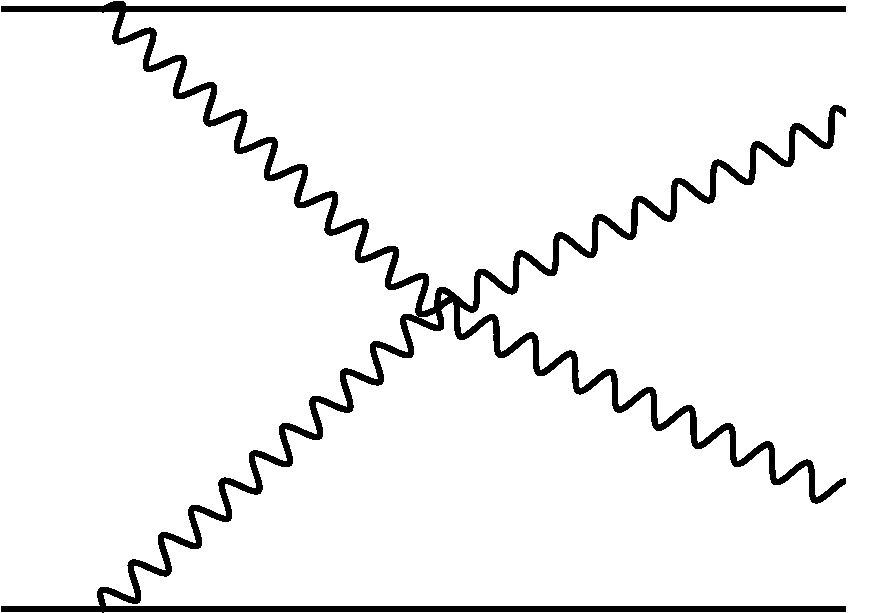
\includegraphics[width=0.3\textwidth,keepaspectratio]{figures/samples/feynVBS2.pdf}
}
\subfigure[]{
 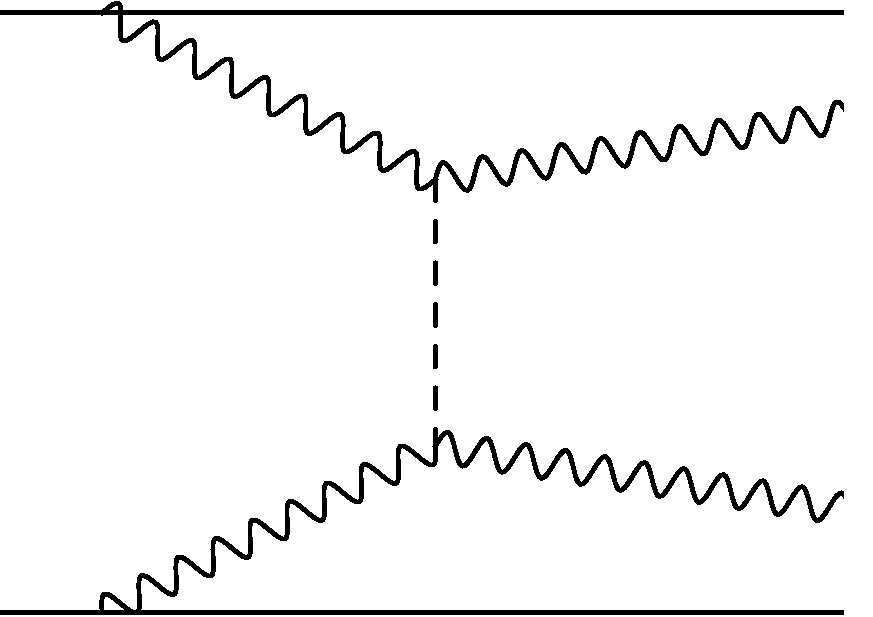
\includegraphics[width=0.3\textwidth,keepaspectratio]{figures/samples/feynVBS1.pdf}
}
\subfigure[]{
 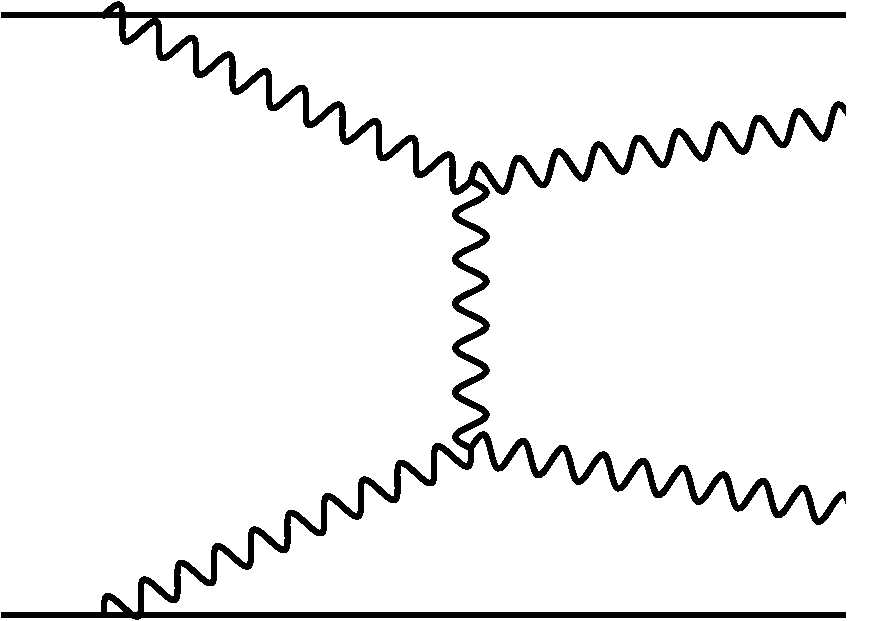
\includegraphics[width=0.3\textwidth,keepaspectratio]{figures/samples/feynVBS3.pdf}
}
\subfigure[]{
 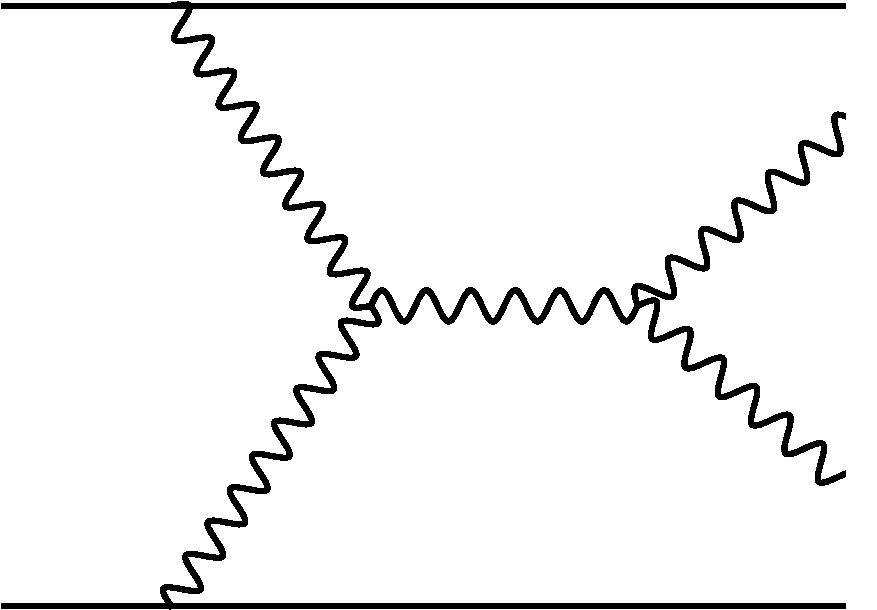
\includegraphics[width=0.3\textwidth,keepaspectratio]{figures/samples/feynVBS4.pdf}
}
\subfigure[]{
 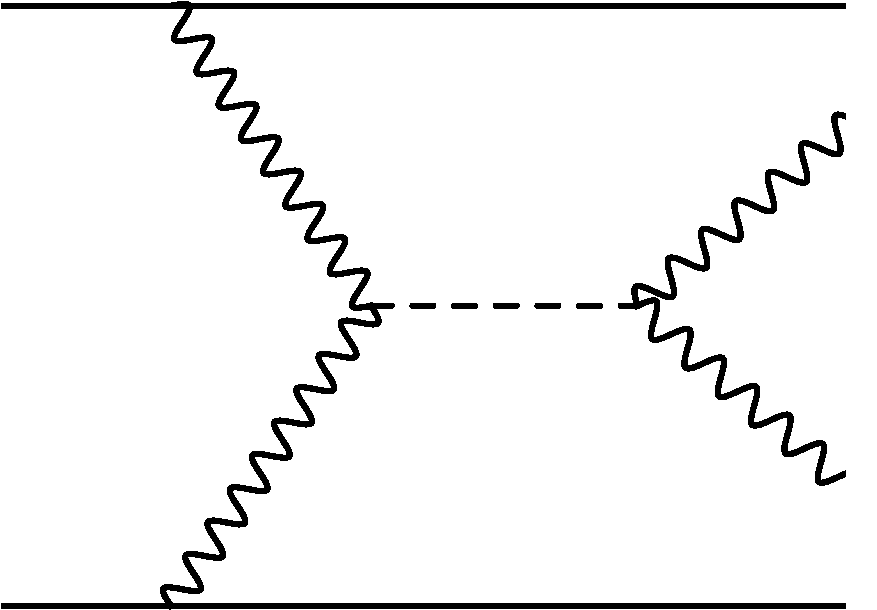
\includegraphics[width=0.3\textwidth,keepaspectratio]{figures/samples/feynVBS5.pdf}
}
\caption{
Examples of VBS diagrams that contribute to the signal.  Note that not all VBS diagrams contain quartic gauge couplings.
The dashed line represents the Higgs boson.  These and other Feynman diagrams in this note are made
using the JaxoDraw~\cite{Binosi:2003yf} program. The decays of the bosons are not shown.
}
\label{fig:feynmanVBS}
\end{center}
\end{figure}

%% feynman diagrams, non-VBS
%
\begin{figure}[tbp]
\begin{center}
\subfigure[]{
 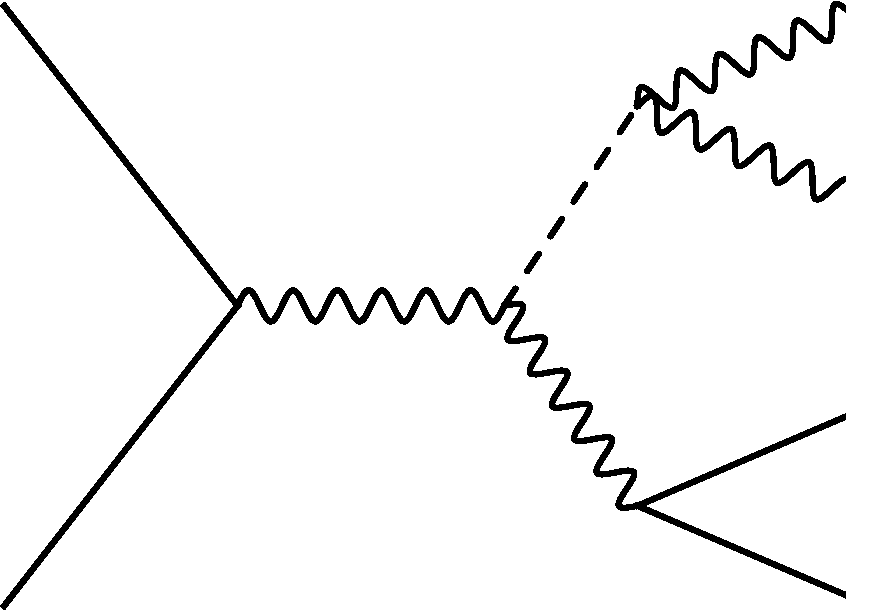
\includegraphics[width=0.3\textwidth,keepaspectratio]{figures/samples/feynEWKnonVBS3.pdf}
}
\subfigure[\label{subfig:feynEWKnonVBSb}]{
 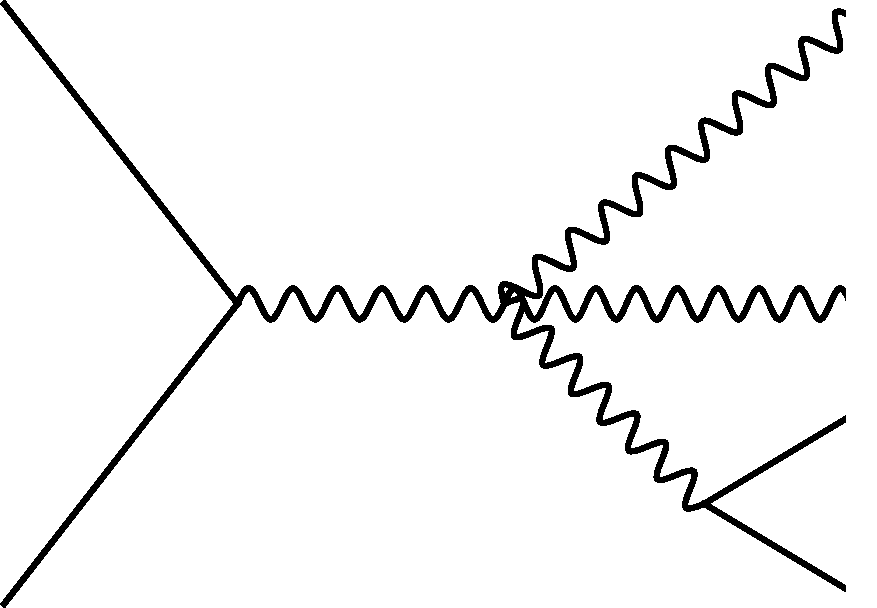
\includegraphics[width=0.3\textwidth,keepaspectratio]{figures/samples/feynEWKnonVBS4.pdf}
}
\subfigure[]{
 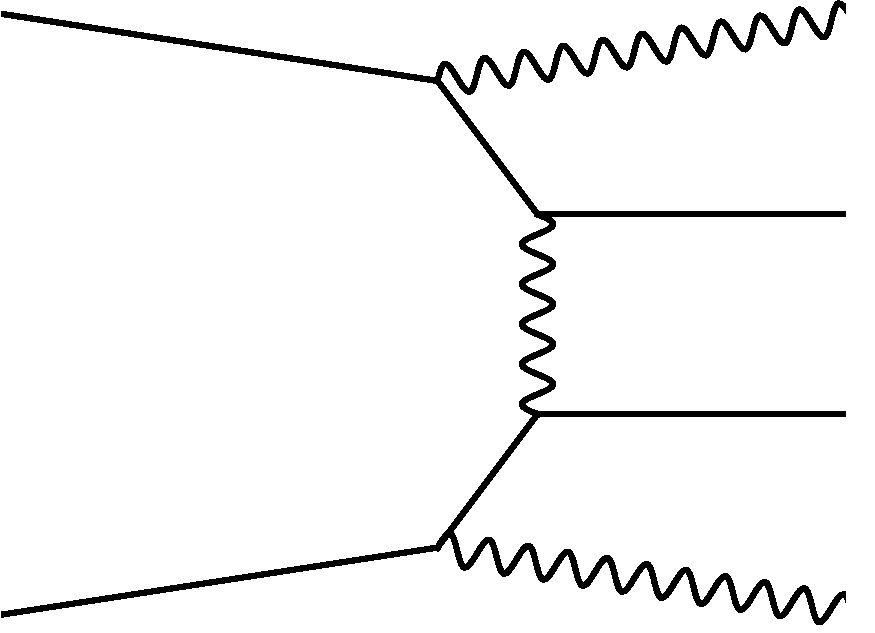
\includegraphics[width=0.3\textwidth,keepaspectratio]{figures/samples/feynEWKnonVBS5.pdf}
}
\subfigure[]{
 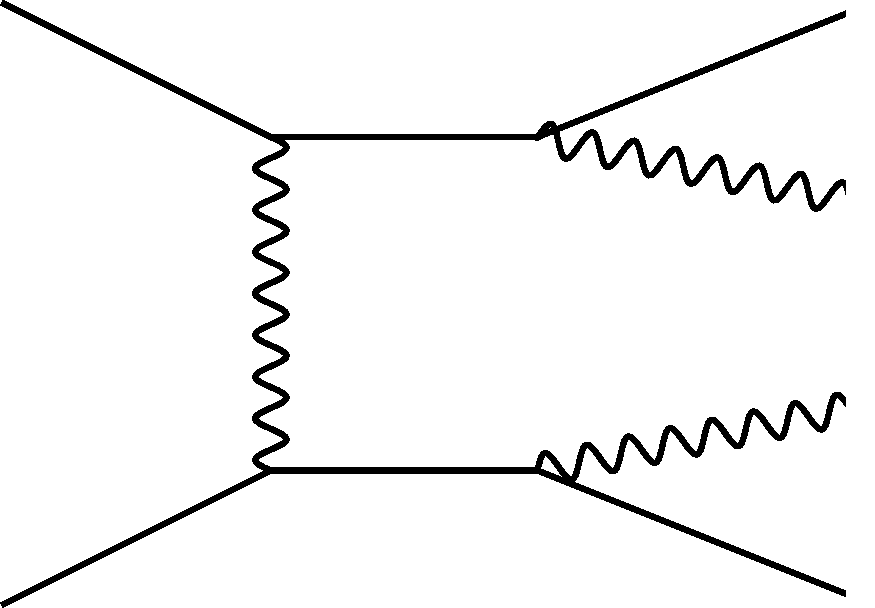
\includegraphics[width=0.3\textwidth,keepaspectratio]{figures/samples/feynEWKnonVBS6.pdf}
}
\subfigure[]{
 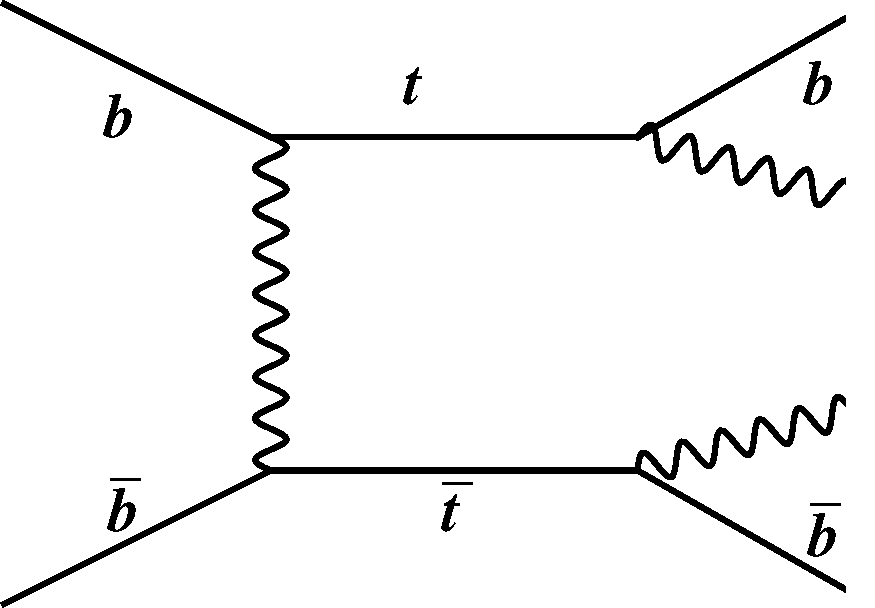
\includegraphics[width=0.3\textwidth,keepaspectratio]{figures/samples/feynEWKnonVBS1.pdf}
}
\subfigure[]{
 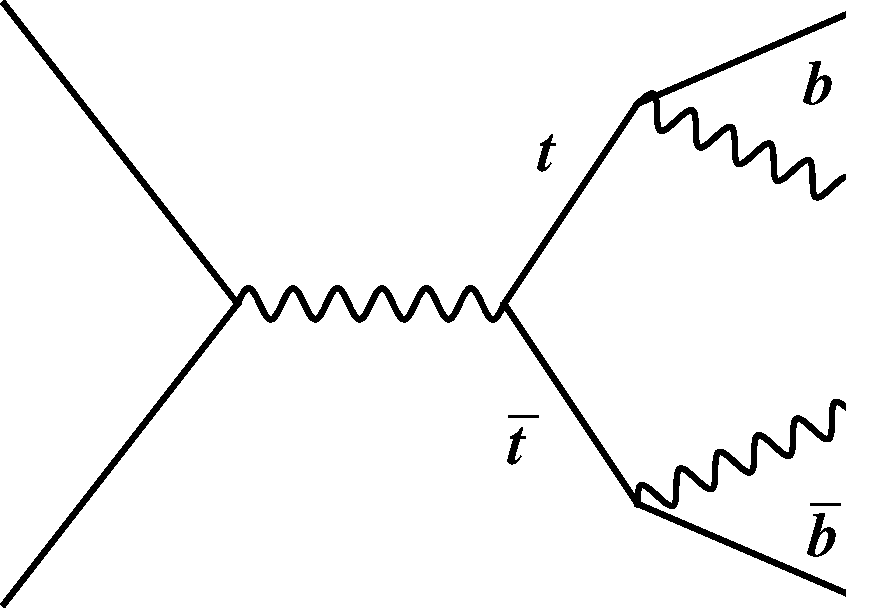
\includegraphics[width=0.3\textwidth,keepaspectratio]{figures/samples/feynEWKnonVBS2.pdf}
}
\subfigure[]{
 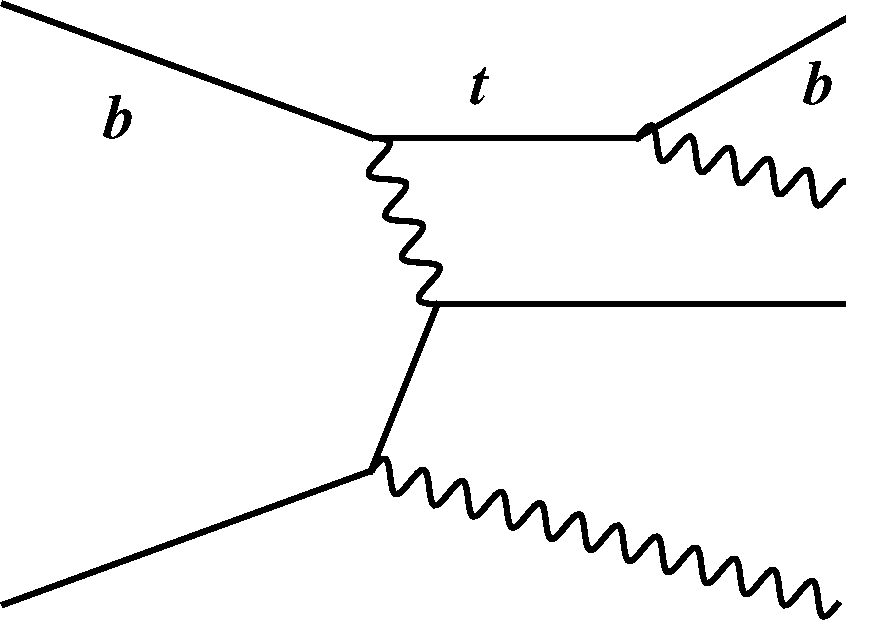
\includegraphics[width=0.3\textwidth,keepaspectratio]{figures/samples/feynEWKnonVBS7.pdf}
}
\caption{
Examples of non-VBS $\mathcal{O}(\alpha_{EW}^6)$ diagrams that contribute to the signal. The decays of the bosons are not
explicitly shown, but the counting of powers of $\alpha$ includes the boson decays.
}
\label{fig:feynmanEWKnonVBS}
\end{center}
\end{figure}

%% feynman diagram, tZb
\begin{figure}[tbp]
\begin{center}
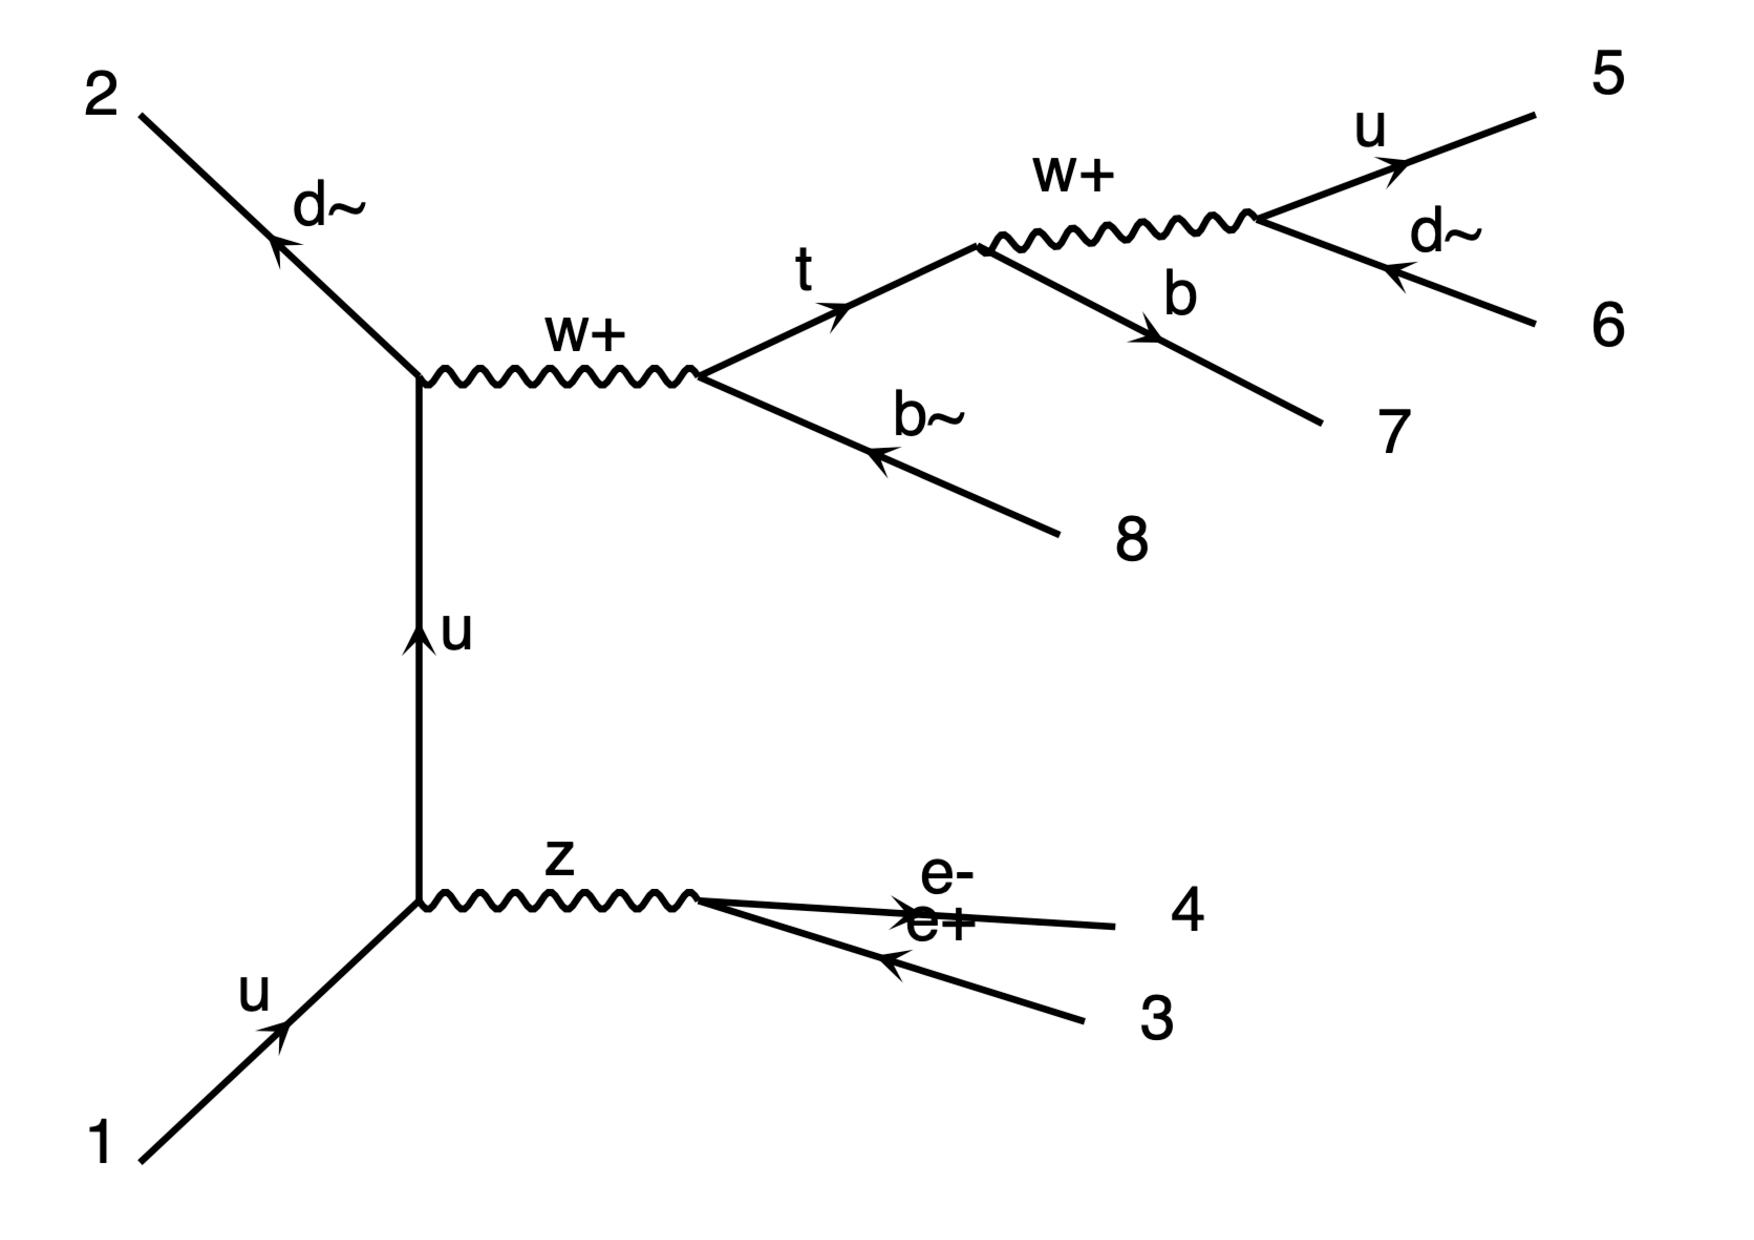
\includegraphics[width=0.3\textwidth,keepaspectratio]{figures/samples/feynEWKnonVBStZb.pdf}
\caption{
The example of the tZb diagram, which included in non-VBS $\mathcal{O}(\alpha_{EW}^6)$ diagrams.
}
\label{fig:feynmantZb}
\end{center}
\end{figure}

%% feynman diagrams, QCD
%
\begin{figure}[tbp]
\begin{center}
\subfigure[]{
 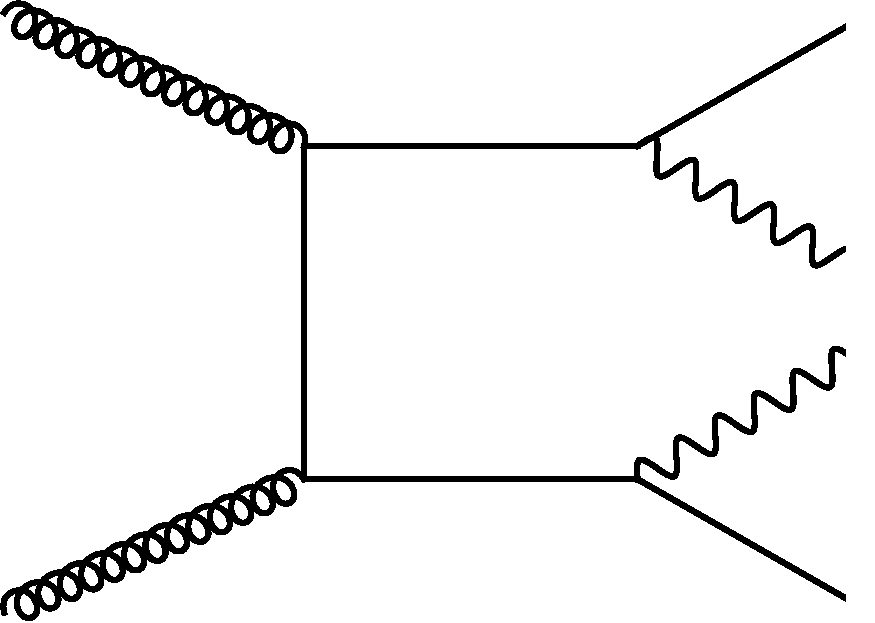
\includegraphics[width=0.3\textwidth,keepaspectratio]{figures/samples/feynQCD3.pdf}
}
\subfigure[]{
 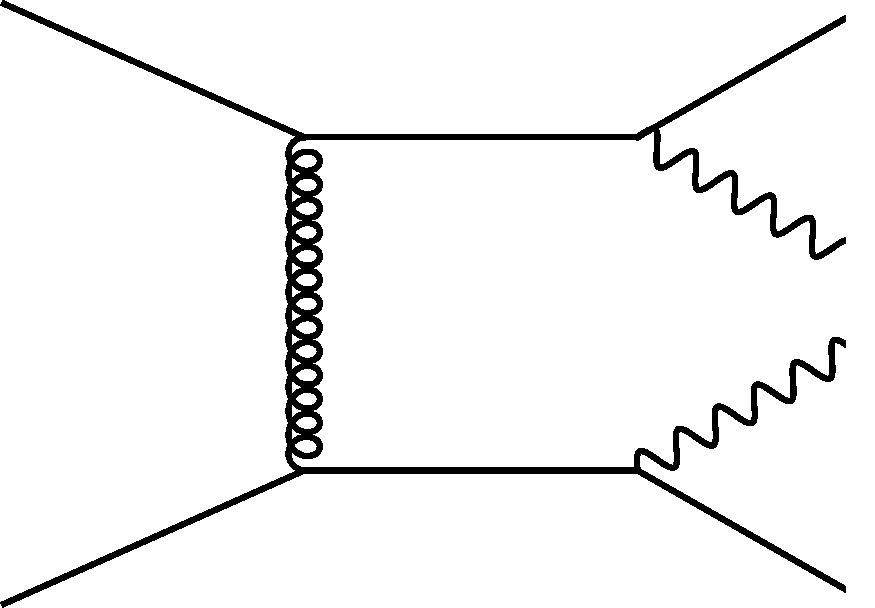
\includegraphics[width=0.3\textwidth,keepaspectratio]{figures/samples/feynQCD4.pdf}
}
\subfigure[]{
 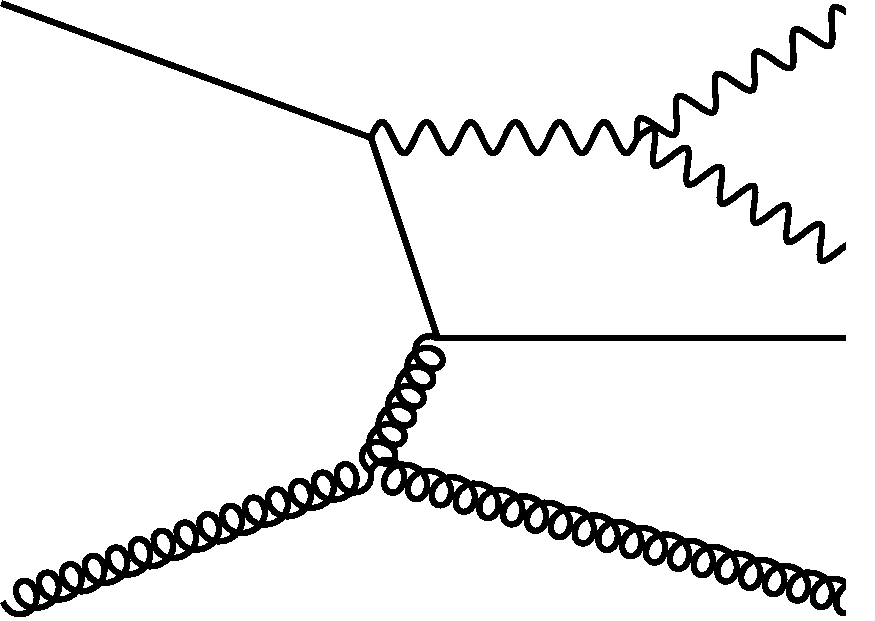
\includegraphics[width=0.3\textwidth,keepaspectratio]{figures/samples/feynQCD5.pdf}
}
\subfigure[]{
 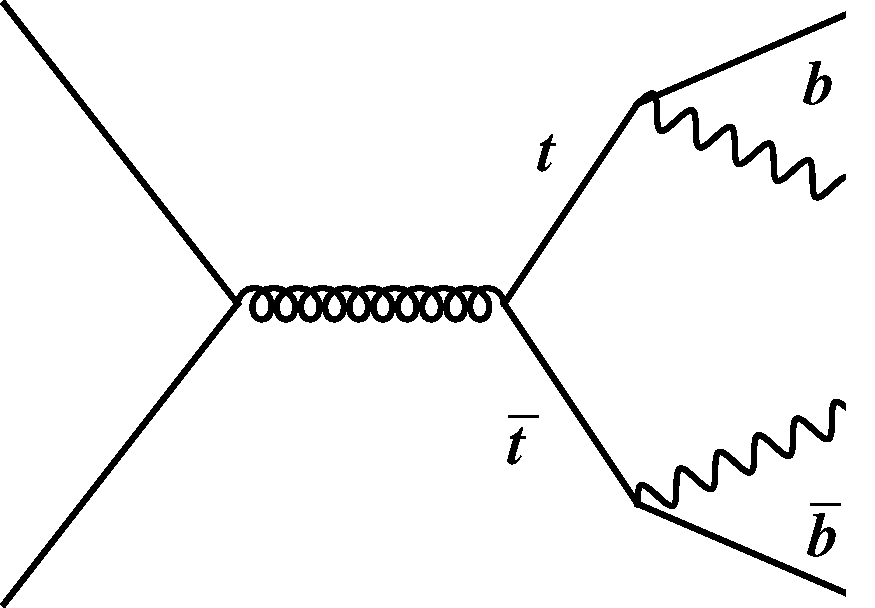
\includegraphics[width=0.3\textwidth,keepaspectratio]{figures/samples/feynQCD1.pdf}
}
\subfigure[]{
 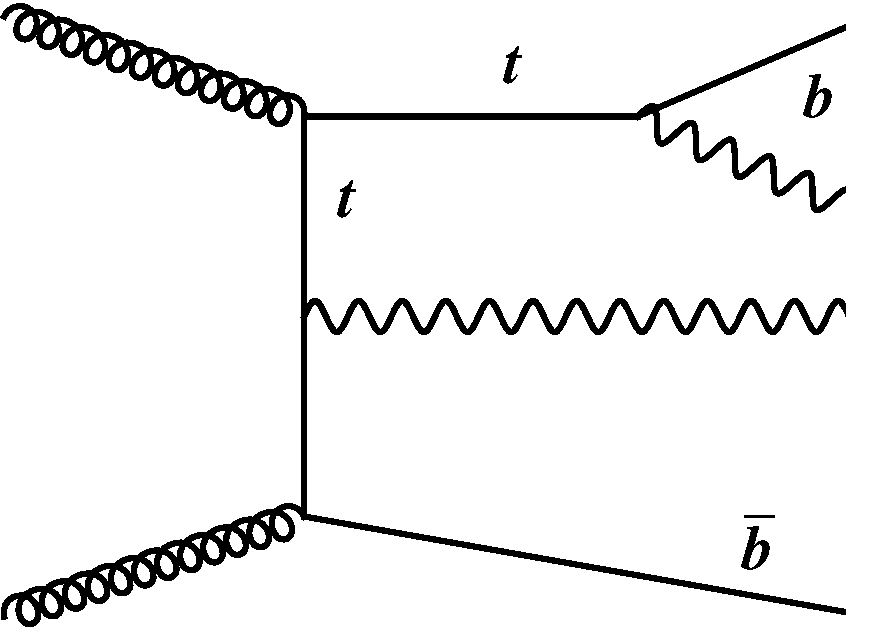
\includegraphics[width=0.3\textwidth,keepaspectratio]{figures/samples/feynQCD2.pdf}
}
\caption{
Examples of $\mathcal{O}(\alpha_{EW}^4 \alpha_{S}^2)$ diagrams that lead to the $VV$+2parton final state. These
are not included in the signal definition.  The decays of the bosons are not
explicitly shown, but the counting of powers of $\alpha$ includes the boson decays.
}
\label{fig:feynmanQCD}
\end{center}
\end{figure}



\section{Anomalous Quartic Gauge Coupling and Effective Field Theory}

To model possible aQGC effect in the VBS process, the Eboli model \cite{eboli2006p} which introduces 21 new dim-8 operators which satisfy the SM $SU(2)\times U(1)_Y$ symmetry is used.
Of these operators, 19 can effect the semileptonic VBS final state.
As typical for EFT expansions, the modified lagrangian with these new operators $\mathcal{L}_n$ and corresponding Wilson coeffiencts $c_n$ and UV scale $\Lambda$ is:
\begin{equation*}
  \mathcal{L}=\mathcal{L}_{sm}+\sum_{n}\frac{c_n}{\Lambda^{4}}\mathcal{L}_n
\end{equation*}

In generality, the matrix-element of a SM process with the addition of new EFT contributions can be written as:
\begin{equation}
  |A_{SM}+c_iA_i|=|A_{SM}^2|+\sum\limits_i c_i^2|A_{i}^2|+ \sum\limits_i 2 c_i \mathrm{Re}(A_{SM}^\star A_i) +\sum\limits_{i\neq j} c_i c_j \mathrm{Re}(A_i^\star A_j)
\end{equation}
where $|A_SM|^2$ is the SM matrix element, $|A_{i}^2|$ represents the pure-EFT matrix element, $2 \mathrm{Re}(A_{SM}^\star A_i)$ is their corresponding interference term, and $\mathrm{Re}(A_i^\star A_j)$ is the possible interference between EFT amplitudes.
This structure can be exploited in recent MadGraph5\_aMC@NLO versions which allows the specific generation of each of these terms individually, known as the matrix-element decomposition method.

Typically one would need to generate a series of samples for each operator $A_i$ at different $c_i$ values, to derive a series of template functions for $|A_{SM}+c_iA_i|$ which would need to be interpolated between for arbitrary $c_i$. Generating samples with the decomposition method greatly simplifies this procedure as one only now needs to generate for each operator $A_i$ the corresponding pure-EFT and interference terms (as well as cross-interference terms if needed). These templates can then be scaled either quadratically or linear with the corresponding $c_i$ values to generate the required full template $|A_{SM}+c_iA_i|$.

The Eboli dim-8 EFT processes are modeled using MadGraph5\_aMC@NLO v2.7.2~\cite{Alwall:2014hca} at LO with the  \textsc{NNPDF30LO} PDF set~\cite{Ball:2012cx} plus \PYTHIA8.244~\cite{Sjostrand:2007gs} for fragmentation.
The matrix-element calculation produces two on-shell $W/Z$ bosons, which are subsequently decayed with \textsc{Madspin}~\cite{Artoisenet:2012st} to simulate the leptonic and hadronic decays of the bosons.
The use of Madspin is required for use of the matrix-element weighting and requires separate generation for each weak isospin state of the boson (i.e the following processes are simulated separately: $W^+W^-$, $W^+W^+$, $W^-W^-$, $W^+Z$, $W^-Z$, $ZZ$).
Each of the 19 contributing operators, across the 6 intermediate diboson state processes and 3 final semileptonic final state processes are generated separately for the pure-BSM and interference term.



